\documentclass{article}
	\def\papertitle{Under-ice acoustic navigation using real time model-aided range estimation}
	\def\authors{E. Bhatt, O. V\'{i}quez, H. Schmidt}
	\def\journal{Journal of the Acoustical Society of America}
	\def\doi{}

% Define title defaults if not defined by user
\providecommand{\lettertitle}{Author Response to Reviews of}
\providecommand{\papertitle}{Title}
\providecommand{\authors}{Authors}
\providecommand{\journal}{Journal}

%% CROSS REFERENCE TO ORIGINAL DOCUMENT

% if you just use cite
% \usepackage{xr}
% \externaldocument[v1-]{pathToDoc}
% in doc, do \ref{v1-sec:intro}

% if you use hyperref
\usepackage{xr-hyper}
\usepackage[hidelinks]{hyperref}
\makeatletter
  \long\def\myempty{}
  \def\XR@addURL#1{\XR@@dURL#1\myempty{}{}{}{}{}\\}
  \def\XR@@dURL#1#2#3#4#5#6#7\\{%
    {#1}{#2}%
    \ifx\myempty#6\@empty
      {#3}{#4}{\XR@URL}%
    \else
    \fi
  }
\makeatother
\externaldocument[v1:]{../../manuscript/preprint}

\usepackage[includeheadfoot,top=20mm, bottom=20mm, footskip=2.5cm]{geometry}

%% CONTAINS EVERYTHING COMMON TO BOTH DOCUMENTS

% TYPOGRAPHY
\usepackage{cmbright}
\usepackage{amssymb,amsmath}
\usepackage{microtype}
\usepackage[utf8]{inputenc}

% MISC
\usepackage{graphicx}
\usepackage{soul} % Highlight using \hl{}

% TABLE
\usepackage{adjustbox} % center large tables across textwidth by surrounding tabular with \begin{adjustbox}{center}
\renewcommand{\arraystretch}{1.5} % enlarge spacing between rows
\usepackage{caption} 
\captionsetup[table]{skip=10pt} % enlarge spacing between caption and table

%% SECTION STYLES

\usepackage{titlesec}

% section
\titleformat{\section}{\pagebreak \normalfont\LARGE}{\makebox[0pt][r]{\bf \thesection.\hspace{4mm}}}{0em}{\bfseries}
%\titleformat*{\section}{\pagebreak \LARGE\bfseries}

% subsection

\titleformat{\subsection}{\normalfont}{\makebox[0pt][r]{\bf \thesubsection.\hspace{4mm}}}{0em}{\bfseries}
\titlespacing{\subsection}{0em}{1em}{-0.3em} % left before after
\titleformat*{\subsection}{\large\bfseries}
\titlespacing*{\subsection}
{0em}{1em}{1em}

% subsubsection
\titlespacing*{\subsubsection}
{0em}{0.5em}{0.5em}
\renewcommand\thesubsubsection{\arabic{section}.\arabic{subsubsection}}

%% PARAGRAPH STYLES

\setlength{\parskip}{0.6\baselineskip}%
\setlength{\parindent}{0pt}%

%% QUOTATION STYLES

\usepackage{framed}
\let\oldquote=\quote
\let\endoldquote=\endquote
\renewenvironment{quote}{\begin{fquote}\advance\leftmargini -2.4em\begin{oldquote}}{\end{oldquote}\end{fquote}}

\usepackage{xcolor}
\newenvironment{fquote}
  {\def\FrameCommand{
	\fboxsep=0.6em % box to text padding
	\fcolorbox{black}{white}}%
	% the "2" can be changed to make the box smaller
    \MakeFramed {\advance\hsize-2\width \FrameRestore}
    \begin{minipage}{\linewidth}
  }
  {\end{minipage}\endMakeFramed}

%% TABLE STYLES

\let\oldtabular=\tabular
\let\endoldtabular=\endtabular
\renewenvironment{tabular}[1]{\begin{adjustbox}{center}\begin{oldtabular}{#1}}{\end{oldtabular}\end{adjustbox}}

%% MACROS FOR FORMATTING NICELY

% common
\usepackage{mdframed}
\newmdenv[
  topline=false,
  bottomline=false,
  rightline=false
]{sideline}

\newcommand{\ebline}[1]{
	\begin{sideline}
	\begin{em}
	#1
	\end{em}
	\end{sideline}
}

%% MACROS FOR CROSS REFERENCING %%
\newcommand{\llabel}[1]{\hypertarget{llineno:#1}{\linelabel{#1}}}

% rebuttal-letter
\usepackage{ifmtarg}% http://ctan.org/pkg/ifmtarg
\makeatletter
\newcommand{\formatLineTracking}[2]{%
  \@ifmtarg{#2}{\subsubsection{#1}}{\subsubsection{#1 \textrightarrow ~\ref*{#2}~(pg. \pageref*{#2})}}
  }
\makeatother

\newcommand{\lreviewer}[3]{
  \formatLineTracking{#1}{#2}
	\ebline{#3}
}

\newcommand{\reviewer}[2]{
  \subsubsection{#1}
  \ebline{#2}
}

% reviewer-letter
\newcommand{\bigcomment}[1]{
\subsection{}
\vspace{-3em}
#1
}

%%DIF PREAMBLE EXTENSION ADDED BY LATEXDIFF
%% DIF UNDERLINE PREAMBLE %DIF PREAMBLE
\RequirePackage[normalem]{ulem} %DIF PREAMBLE
\RequirePackage{color}\definecolor{RED}{rgb}{1,0,0}\definecolor{BLUE}{rgb}{0,0,1} %DIF PREAMBLE
\providecommand{\DIFadd}[1]{{\protect\color{blue}\uwave{#1}}} %DIF PREAMBLE
\providecommand{\DIFdel}[1]{{\protect\color{red}\sout{#1}}}                     %DIF PREAMBLE
%DIF SAFE PREAMBLE %DIF PREAMBLE
\providecommand{\DIFaddbegin}{} %DIF PREAMBLE
\providecommand{\DIFaddend}{} %DIF PREAMBLE
\providecommand{\DIFdelbegin}{} %DIF PREAMBLE
\providecommand{\DIFdelend}{} %DIF PREAMBLE
%DIF FLOATSAFE PREAMBLE %DIF PREAMBLE
\providecommand{\DIFaddFL}[1]{\DIFadd{#1}} %DIF PREAMBLE
\providecommand{\DIFdelFL}[1]{\DIFdel{#1}} %DIF PREAMBLE
\providecommand{\DIFaddbeginFL}{} %DIF PREAMBLE
\providecommand{\DIFaddendFL}{} %DIF PREAMBLE
\providecommand{\DIFdelbeginFL}{} %DIF PREAMBLE
\providecommand{\DIFdelendFL}{} %DIF PREAMBLE
%DIF END PREAMBLE EXTENSION ADDED BY LATEXDIFF

%% RANDO TEXT FOR EXAMPLE
\usepackage{lipsum}

%% CHECKS IF THINGS ARE EMPTY
\usepackage{etoolbox}

\begin{document}

% Make title
{\Large\bf \lettertitle}\\[1em]
{\huge \papertitle}\\[1em]
{\authors}\\
{\emph{\journal}}\ifdefempty{\doi}{}{, \texttt{doi:\doi}}\\
\hrule

% Legend
% \hfill {\vline ~\textit{Reviewer Comment}, Author Response, \(\quad\square\) Manuscript text

\begin{flushright}
\vspace{-1em}
\vline ~ \emph{Reviewer Comment} \\
Author Response \\
$\square$ Manuscript Text
\end{flushright}

% table of contents
\renewcommand{\contentsname}{}
\begingroup
\let\pagebreak\relax
\setcounter{tocdepth}{1}
\tableofcontents
\endgroup


\section*{Cover Letter}
Dear Editors,

We thank the reviewers and editor for their thoughtful feedback and comments in improving this work.
We have refashioned the abstract and introduction to better elucidate the motivation for this work as a model-aided component for LBL navigation in total under-ice conditions, which could be further generalized for any acoustic environment.
Based on several suggestions, we have restructured the manuscript and separated the real-time from the post-processed range estimation results.
Our original revision aimed to contextualize the range estimation results as a proxy for navigation.
Given several points from the reviewers and editor about the lack of this transferability, we have added AUV post-processed navigation results as well.
The real-time results are also covered but have no GNSS ground truth to compare to.

For clarity, we also more prominently establish definitions for navigation, positioning, and re-positioning to better contextualize our results and contributions, based on this discussion in Howe et al (2019) \emph{Observing the Oceans Acoustically} (and many others):

\begin{quote} 
PNT is a combination of three distinct, constituent capabilities:

\begin{enumerate}
	\item Positioning is the ability to accurately and precisely determine one’s location referenced to a standard geodetic system;
	\item Navigation is the ability to determine current and desired position (relative or absolute) and apply corrections to course, orientation, and speed to attain a desired position anywhere in the domain of concern; 
	\item Timing is the ability to acquire and maintain accurate and precise time anywhere in the domain of interest within user-defined timeliness parameters; it also includes time transfer.
\end{enumerate}

Navigation is real time and necessarily depends on positioning, and positioning depends on timing.
\end{quote}

Given the tension of evaluating our travel time to range conversion on events between LBL beacons in real time and post-processing, we further delineate that, in this work, positioning is in real time and re-positioning is post-processed.
We have also added re-positioning trilateration results, processed with only the available field data and algorithms that could be performed in real time, to emulate navigation performance.

The rebuttal letter is organized with sections delineated by the review document and email. We look forward to your comments and the opportunity to continue improving this manuscript for potential publication in JASA. Thank you again for your time and consideration.

We also thank JASA for a generous extension given that the corresponding author started (and is still on) parental leave.

Sincerely,

Dr. EeShan Bhatt \emph{on behalf of all authors}

% \ref*{v1:test}
% \pageref*{v1:test}
% \formatLineTracking{test}{v1:test}

%% ------- COMMENTS FROM REVIEWER ONE ------ %%
\section{Reviewer One}

	\subsection*{Summary}

	\ebline{This paper demonstrates how a positioning system over \texttt{\small $\sim$}1.5-3 km of range achieves 11 m of positioning uncertainty. The work demonstrates how a single group velocity calculated from acoustic rays predicted by BELLHOP can be used to estimate ranges to be used in a LBL network for positioning. The data presented are from transceivers on fixed ice-tethered buoys but the system could also be implemented on an autonomous underwater vehicle.}

	This summary captures key results presented in the paper. However, we note that the system was successfully deployed on an underwater vehicle during ICEX20. The results from this work are specifically limited to the methodology behind calculating a single group velocity, which we attempt to quantify through beacon-to-beacon communications with known GNSS timestamps.

	\subsection*{Overall Comments}

	\reviewer{}{The claims made in the abstract need to be better supported by the data presented or else tempered a bit. What is demonstrated here is not real-time navigation on a vehicle, but calculation of a handful of short fixed ranges from ice-tethered buoys. The limited data presented here begs more discussion with regards to how applicable the algorithm would be in normal vehicle operation and to navigation of the vehicle, as there were limited ranges between the beacons. What depths does the vehicle typically operate at and what is the maximum range from the beacons?  The abstract stresses real-time results, but the real-time results are just 3 paragraphs, and the paper mostly concentrates on post-processing results.} \label{1dot1}

	We have adjusted the claims made in the abstract (and throughout the paper) and hope we have presented data to better support them as well. 
	While we initially aimed to contextualize the calculation of a handful of short fixed ranges between ice-tethered buoys as the proxy for navigation, we agree with the reviewer that this is a severe shortcoming. Accordingly, we added the same analysis for the AUV run in ICEX20. 

	We have also addressed valid questions about transferability to other vehicle operations in the discussion (line \ref{v1:1.1}).

	\reviewer{}{The hypothesis is stated in the discussion section lines 515 and following: “We hypothesize and validate that the embedded stochastic prediction of a single group velocity is a smoothly varying function of range, source, and receiver depth pairings as well as multipath structure.”  I am not convinced that the few short fixed ranges presented here validate this hypothesis.  Lines 248 and following indicate how the system should track a continuously changing group velocity, but this is not demonstrated with the few fixed ranges presented here.  Also, it would be good to state this hypothesis more clearly earlier in the manuscript.}

	We agree that a few short fixed ranges do not validate this hypothesis. With the overarching motivation and design of LBL navigation, however, we have recast this hypothesis as an assumption (line \ref{v1:2.10}).

	\reviewer{}{The introduction and conclusion sections should be tightened up to clarify the state of the art in various arenas of underwater vehicle navigation and how this work fits in.

	The error metrics presented here should be specifically compared with other positioning systems or algorithms over similar spatial scales that do not integrate the ray propagation physics.

	Various ranging and positioning methods are referenced, but the narrative jumps between different types of AUVs and implementations and between scales of a few kilometers and hundreds of kilometers. This should be discussed in terms of range, vehicle, and propagation conditions. 

	Line 176 mentions that the SSP and the physics of ray refraction are often overlooked in positioning algorithms; this is, I presume, referring to real-time results or short-range results, but doesn’t specifically say this.}

	We believe we have tightened up the introduction and conclusion sections by focusing on this work as a model-aided augmentation to an LBL system.
	Then we specifically talk about AUV-LBL systems deployed in under-ice conditions.
	This focus presents the narrative more linearly, instead of it feeling like it jumps between different types of deployments.

	The error metrics are presented as RMS m. Other positioning systems at similar scales are now covered in the introduction (line \ref{v1:1.3a}). We have also added an isovelocity case for fairer comparison to other smaller spatial scale AUV deployments and the proposed method in this manuscript. 

	Thank you for the suggestion to discuss in terms of range, vehicle, and propagation conditions. We have not done this explicitly but taken care to illustrate the differences, and what parts we are comparing.
	
	Lastly, yes, we did mean real-time navigation, but have removed the line in question.

	\reviewer{}{Related to the point above, the introduction should make clear what type of vehicles the proposed method of navigation is applicable to and over what ranges. The authors do start to do this when they note that a shallow receiver depth enables the estimation method (line 274), but should more directly specify under what conditions the proposed algorithm is applicable.  In the Discussion section, there is an implication that this method of using a single group velocity could be applied to mesoscale operations but should acknowledge that propagation at these larger scales results in arrivals that are spread over several seconds including multiple modal arrivals with varying group velocities.  This method would presumably result in errors much higher than 11m….how might that scale?}

	{\color{blue} COME BACK TO THIS.}

	\reviewer{}{I understand what the authors are referencing when they use the term “group velocity” but I think this term should be used a bit more carefully.  Group velocities are often associated with modal propagation in which each mode has a distinct group velocity.  The goal in this work is to determine a single group velocity by taking a power weighted average of several different ray arrivals to derive range.  This is addressed somewhat in lines 395 and following, but I think it would be appropriate to expand on this discussion and move it up.  Lines 235 and following state “the variation of horizontal group velocity from any source-receiver pair is the fundamental challenge to implement GPS-like navigation in an LBL navigation paradigm…” this statement could use some clarification.  Also, perhaps change the axis on Figure 5 to read something like ‘implied group velocity.”} \label{1dot5}

	Thank you, these are all excellent suggestions. Instead of ``group velocity'' we use a combination of ``effective sound speed'', noted by $c$. The statement in question has been rewritten to talk about a single sound speed compensating for ray refraction and reflection, and is on line \ref{v1:1.5}.

	\reviewer{}{As written, this manuscript seems more suited to an ocean engineering journal.  For a JASA audience, this should be more focused on the acoustics.  Perhaps I missed it, but I didn’t see that the manuscript even mentioned the frequencies or waveforms that were used in the experiment.  I’d suggest, for example, less emphasis on which options were toggled on/off or triggered (e.g. line 186, 196, 241, 254 ) and more on, for example, why specific depths were chosen and how they provide better coverage due to the acoustic shadow zone (e.g., Line 155), or how the specific rays were eliminated by the filtering (Line 232). Lines 370-372 state “The increased error for these reciprocal transmission paths is most likely driven by the computational artifacts encountered when propagating through the steep sound speed gradients of the lens and through the shadow zone.“ The authors might consider providing more information on these artifacts.}\label{1dot6}

	Agreed on all points. The frequencies are now included in the ICNN description (line \ref{v1:1.6a}). The discussion of which options were toggled on and off has been removed in favor of a in depth discussion of shadow zone, computational artifacts, and eigenray filtering in Section III.C, starting line \ref{v1:1.6b}.

	\reviewer{}{There seems to be a somewhat outsized discussion of GPS drift, but I didn’t see how the GPS uncertainty was directly applied to the uncertainty values presented in the paper.  I’d suggest condensing this section.}

	This section has been significantly condensed and is now Section V.C, starting line \ref{v1:1.7}. The GPS uncertainty is now directly compared to the uncertainty from beacon-to-beacon re-positioning and AUV re-navigation.

	\subsection*{Specific Comments}

	\lreviewer{line 226}{v1:1.8}
	{In the section describing post-processing analysis, the authors bring up that the processing was designed to mirror information available on a submarine – modeled data, historical data, and in situ data.  This is a nice rationale for the analysis, and I’d suggest highlighting this in the introduction.}

	Thank you. This is now included in the ICEX20 experiment description, Section II.

	\lreviewer{}{}{How long was the experiment from start to finish, and how much did the sound speed profile change over the duration of the experiment?}

	This is a great question! The experiment was four days. The last few CTDs showed a significantly weaker duct than those at the beginning. The local sound speed maxima went from 1447 m/s at 40 m in depth to 1442 m/s at 60 m in depth. Related work on the environmental adaptivity has just been accepted in IEEE JOE.

	\lreviewer{}{}{What is the magnitude of the uncertainty in the position of the transceivers relative to the GPS positions measured at the surface? Presumably the transceivers particularly at 90 m depth could move from the lat/lon position of the GPS receivers at the surface.}

	We assume negligible uncertainty in the position of the modems relative to the surface expression given that the ice drift rate was unusually low, roughly 0.7 cm/s. This is now included on line \ref{v1:1.10}.

	\lreviewer{lines 40-42}{v1:1.11}{Note ranging via one way travel times that have been used prior to the advent of the micro-modem, for example RAFOS.}

	Thank you. We have included this point and make the distinction that RAFOS floats are re-positioned.

	\lreviewer{line 192}{v1:1.12}{Clarify what you mean when you state that the transmit and receive layers are independent? Also, the discussions of physical and virtual layers are confusing. I think everything is there, but reorganization would make this more clear. Consider moving up the paragraph starting at line 203.}

	We have removed the jargon of the physical and virtual layers in favor of a more streamlined explanation. The transmit and receive layers are activated independently.

	\lreviewer{line 205}{v1:1.13}{What do you mean that the coordinate system is range independent?}
	We meant that the analysis of beacon-to-beacon connections is presented in r/z, not x/y/z. We found this framing awkward as it is more common to say the propagation has a depth dependent sound speed profile with range dependent bathymetry.

	\lreviewer{line 222}{v1:1.14}{Could you provide more information on the baseline and weighted SSPs. Where did the baseline profile come from?}
	\label{1dot14}

	In anticipation of ICEX20, all of the ITP data for the Beaufort Sea was assimilated. For operation reasons, we designed a system to transmit sound speed updates through digital acoustic message. This system relied on a simple basis function representation of the sound speed and its perturbations. Given the wide range of observed ducted conditions across all ITP data, several basis sets were created, corresponding to March of different years. During ICEX20, the data from Mar 2013 was found to be the closest match for observed conditions. The baseline is the mean sound speed from Mar 2013. The weighted is the basis set projection for the CTD taken during ICEX20.

	\lreviewer{line 256}{v1:1.15}{How is the group velocity uncertainty calculated?}
	
	We meant standard deviation, and have changed this accordingly. It is equation 2. 

	\lreviewer{line 231}{v1:1.16}{Quantify the travel-time proximity to recorded data that was used to filter the eigenrays.}

	It was a one millisecond filter to cluster distinct arrivals.

	\lreviewer{lines 260, 303-305}{v1:1.17}{Please provide more information on the BELLHOP implementation.   Line 260 indicates a sparse grid.  From lines 303-305 do I understand that the grid is 1m in range and 2 m in depth?}

	This was not clear. We meant sparse as in not full-field, which we agree is misleading. The grid is 121 points with 1 m spacing in range and 2 spacing m in depth.

	\lreviewer{line 309}{v1:1.18}{Suggest re-writing this sentence for clarity: “As expected, the algorithm is generally overestimating range as it resolves a direct path that does not represent the actual arrival.”}

	This has been rewritten as ``The algorithm generally overestimates pseudoranges because it resolves the effective sound speed for the most direct path.''

	\lreviewer{line 364}{v1:1.19}{Could use a figure reference.}

	We have added a figure reference.

	\lreviewer{line 562}{v1:1.20}{I don’t agree that many approaches to underwater navigation combine it with acoustic tomography.}

	We agree, ``many'' misdirects the current state of the art. The benefit of concurrent navigation and tomography has been discussed, but it remains to be used as a standard technique.

	\lreviewer{Figure 1}{v1:fig:vehicleRecovery}{Figure 1 is a nice picture showing the vehicle, which motivates the work presented here, but was not used for collection of any of the data presented.  As it’s not pertinent to the data presented here, I’d suggest removing this figure or at least combining this figure with Figure 2.}

	Thank you. We have kept this image but added the vehicle track, as it is necessary for the re-navigation analysis as mentioned in Comment \ref{1dot1}.

	\lreviewer{Figure 3}{v1:fig:overview}{Figure 3 tallies the number of successful events, and I think the use of the directional arrows communicates the data well.  How many events are successful in comparison with those that are considered unsuccessful and what generally causes an event to be deemed unsuccessful?}

	Thank you. We have added a successful decoding percentage, defined as the ratio of decoded over detected messages. We have also added the total number of transmissions, so one can see the ratio of detected over transmitted. An event is deemed unsuccessful given any error in the data frame, even if the error has nothing to do with the information necessary for positioning.

	\lreviewer{Figure 5}{v1:fig:gvel-post}{What is the point labeled u=751 m/s that appears to fall around 1424 m/s?}

	That point is an effective sound speed prediction dominated by a bottom bounce. The figure has been changed to include all source depths. Keeping this point in would visually compress the other data. However, it is now discussed narratively, in line \ref{v1:1.23}.

	\lreviewer{Table II}{}{Might this information be portrayed better by a box plot?}

	This table described pseudorange statistics. Given that these are no longer serving as a proxy for navigation, it has been removed. The statistics for re-positioning and re-navigation are now included as histogram-box plots (Figs 11 and 12).

	\subsection*{Minor Edits}

	\lreviewer{Fig. 2 and 3}{}{Fig 2 refers to central node position as Topside and Fig. 3 as Camp Seadragon. Suggest standardizing.}

	Thank you. We have standardized this to Topside.

	\lreviewer{lines 311, 359}{}{'Data' should be plural.}
	Thank you. This has been corrected.

	\lreviewer{Figure 6}{v1:fig:rangeError}{Suggest including receiver depth along with source depth in the title as they are both important in distinguishing between the cases.}

	The source depths have been moved from the column titles to the individual sub-panels.

	\lreviewer{Table I}{}{Table I indicates direction errors are positive. Please note the sign convention in the caption.}

	We have removed the table but discuss this in the text at line \ref{v1:1.28}, and have corrected the convention.

	\lreviewer{Table II}{}{‘range estimation error metrics’ rather than ‘range estimation metrics’?}
	Agreed. While we have removed the table, we have adopted this language.

	\lreviewer{Table II and III}{}{Suggest removing ‘algorithm’ label.  Also substitute ‘MBC’ and ‘NBC’ for minimal and nearest to match the text.}
	Agreed. While we have removed the table in favor of histogram/box plot, we have adopted this language.

	\lreviewer{}{}{There are several figures and tables which are not referenced properly (Line 305, 391, 411)}
	Thank you. This has been corrected and we apologize for the typographical mistakes.

%% ------- COMMENTS FROM REVIEWER TWO ------ %%

\section{Reviewer Two}

	\lreviewer{line 7}{v1:2.1}{'Beaufort Lens' This is not yet a scientific term, suggest finding descriptive terms to use. What comprises the 'lens'? The Pacific Summer Water is the warm layer.}\label{2dot1}

	We have removed the ``Beaufort Lens'' language from the abstract as it may not be self explanatory. However, the Beaufort Lens has been used in the literature (Litvak 2015, Schmidt and Schneider 2016) and in JASA/POMA specifically (Poulsen et al 2016, Chen et al 2019).

	We think of the lens as any feature that introduces significant refraction, such that the term Beaufort Lens is a convenient shorthand for the spatio-temporal variability of the warm water intrusion provided by the Pacific Summer Water Layer that creates two ducts. We prefer this distinction as the lens exists in the oceanographic space but the ducts are acoustic features dependent on source depth and frequency. With this jargon, the lens is susceptible to aberrations from eddies or filaments in the same way that the duct is susceptible to leaking.

	For clarity, we explictly define the Beaufort Lens in the manuscript as discussed here at line \ref{v1:2.1a}.

	\lreviewer{line 10}{v1:2.2}{'GPS aided', do you mean GPS-navigated?}
	We have changed this to ``GPS-linked'' because navigation implies self-movement.

	\lreviewer{line 12}{v1:2.3}{'rival GPS' is a fairly bold statement when GPS is used as ground truth.} \label{2dot3}

	We meant ``rival GPS'' in that the downstream accuracy of the acoustic range estimation method is within the precision of GPS. However, we have amended this framing to say that our best performing acoustic method does not introduce significant additional error than is already documented by GPS puck precision, effectively extending single GPS performance into the shallow water column for a small volume of interest. Given more beacons, there is potential to reduce uncertainty in the same way that differential GPS works. While this refrain is used multiple times in the revised manuscript, please see Section V in particular.

	\lreviewer{line 89}{v1:2.4}{Is the 'lens' the warm water? Or a combination of layers? What does 'lens' mean acoustically? Normally in ocean acoustics people refer to ducts and layers.}

	Please see comment \ref{2dot1}.

	\lreviewer{line 94}{v1:2.5}{Ice Tethered profiler data shows fairly slow variability in space and time in the Beaufort, but changes in characteristics occur as the deep basin transitions to the Chukchi, so what is meant by 'high degree' exactly?}

	ITP data and modeling efforts by Duda et al (2019, 2021) suggest the duct is persistent and widespread but not always continuous in the Beaufort. Of course, it breaks down towards the shallower Chukchi basin. Thus ``high degree'' refers to variance of the observed ducted conditions, i.e., the duct and its acoustic effects can be non-existent, minimal, or drastic.
	This is easily seen by parsing an integral duct parameter, $\kappa$, that measures the area spanning the local sound speed maximum from the lens to its conjugate depth, for all relevant ITP data.

	\begin{figure}[!h]
	\centering
	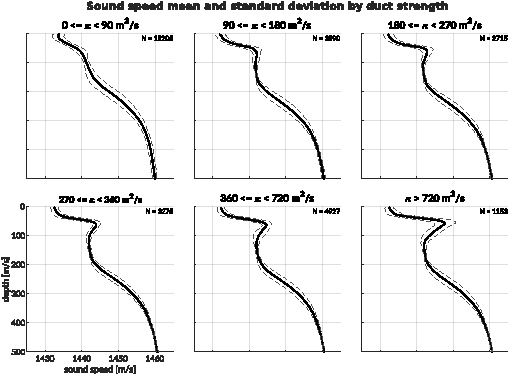
\includegraphics[width=\textwidth]{ssp-ducts-lines}
	\caption*{Adapted from Chapter 3 of Bhatt, E. (2021) An empirical Virtual Ocean framework for environmentally adaptive, embedded acoustic navigation for autonomous underwater vehicles, PhD Thesis.}
	\end{figure}
	\clearpage

	\lreviewer{line 4}{}{Fig 4 - where did the baseline come from (exactly)? What database, etc.}
	Please see Comment \ref{1dot14}.

	\lreviewer{line 224}{v1:2.7}{why did a human have to chose an optimal set of weights? Why not just use the measured SSP, or an average of a few?}

	We have removed this statement, as it is not relevant to the findings of this work. However, the navigation solution existed in tandem with an interactive tactical decision aid (TDA) operated by a Navy submarine officer. A lightweight compression of the sound speed profile was needed to facilitate its update via digital acoustic message. Work about this TDA has been recently accepted for publication in IEEE JOE.

	\lreviewer{line 231}{v1:2.8}{'abundance'. Is there a more precise way to say this? Bellhop does what it is programmed to…}

	Yes, thank you. BELLHOP finds all possible eigenrays given the prescribed launch angles whereas only a few or less (sometimes none) are valid for the travel time of interest.

	\lreviewer{line 241}{v1:2.9}{'modem triggering time', do you mean 'detected arrival time'?}
	Yes. We have changed this accordingly.

	\lreviewer{line 249}{v1:2.10}{Use of the word 'range' for the 'navy range' type of use is intermixed with range as in distance. Suggest not using 'range' and in 'navy range' and saying 'nav' or 'comms' system or network.}

	We have adopted this suggestion and use navigation or communication system instead.

	\lreviewer{line 261}{v1:2.11}{'bring'. Do you mean interpolate?}
	Yes. We have changed this accordingly.

	\lreviewer{line 281}{v1:2.12}{Awkward sentence, either unclear or extremely obvious. "...an acoustic arrival does not always take the direct path from source to the receiver,".}

	We have removed this sentence in favor of discussing ray refraction and reflection.

	\lreviewer{}{}{for both criteria: a graphic that shows the method could be very useful.}

	This is a good point. We hope that the separation of MBC and NBC, as well as the extended discussion in Section III-C, better illustrate both criteria. A visual on its own would be quite similar to the eigenray plots added. However, we are happy to include a graphic showing the method if reviewers find the narrative explanation lacking.

	\lreviewer{line 319}{v1:2.14}{"This is likely driven by the prominence of the duct." Do you mean: consistency of sound speed within the duct where the rays were trapped and thus traveled? Or something else?}

	We mean prominence, often used in peak finding, which would indicate both the considerable sound speed differential and the nearly horizontal slope to the local maxima. This is now explained more clearly and introduced early at line \ref{v1:2.5}.

	\lreviewer{line 410}{}{'anomalous' - does this section need to be included? Or just the issue summarized and noted? Delete the table?}

	{\color{blue} Thank you for this suggestion. We have deleted the table and instead summarized the issue.}

	\lreviewer{lines 585-591}{}{Suggest deleting, not very appropriate for an academic paper.}

	This has been removed.

	\lreviewer{Fig 10}{v1:fig:gvel-post}{Would be good to have some conclusions in addition to the description.}

	This figure has been condensed into the main body of the text alongside conclusions around the effective sound speed estimation.

%% ------- COMMENTS FROM EDITOR ------ %%
\section{Comments from the Editor}

	\reviewer{}
	{Both reviewers recommend that the manuscript be reconsidered after revision based on the reviews, and I concur. The key point of the manuscript seems to be to compare two different approaches to determining an effective sound speed for converting travel times to ranges for use in determining positions by trilateration in an Arctic environment (designated Minimal Bounce Criteria and Nearest Bounce Criteria). The goal is not evident in the abstract and is first more-or-less (but not entirely) clearly stated in Section II (Methods) (lines 174-176). While some discussion of the AUV operations is appropriate to motivate the analysis, the extensive discussion in the Introduction and elsewhere in the manuscript seems unnecessary and inappropriate. The use of jargon from the AUV application (e.g., physical layer, virtual layer) also seems unnecessary.}

	Thank you. The key point of this paper is a model-aided component to the LBL paradigm that we demonstrated in the Beaufort Sea. 
	Because both reviewers and the editor felt the key points were comparing the two different approaches to determine an effective sound speed for converting travel times to ranges, we have significantly restructured the paper to make the narrative clearer. 

	The discussion of AUV operations and jargon from AUV application contextualizes the model-aided component to the LBL paradigm. However, we agree with the Editor that this emphasis can be distracting when used throughout the manuscript.
	We have attempted to use the most direct language possible in each section.
	We hope this revision presents the contributions more clearly and welcome further feedback on this matter. 

	\reviewer{}
	{I agree with Reviewer 1 that the manuscript needs much more information on the acoustic parameters (frequencies, pulse lengths/modulation, ranges, expected travel-time measurement accuracy, etc.). 

	In addition, the ray geometries are quite different for cases in which the source and receiver are both in the surface duct (i.e., 20 and 30 m), both in the Beaufort Duct (for the sound-speed profiles for which it is present) (i.e., 90 m) and one of the source or receiver is in the surface duct and the other is in the Beaufort Duct. The manuscript needs to include some discussion of these different cases.}

	We have now included the information on acoustic parameters in the experiment description. We apologize that this information was ommitted as the manuscript was adapted from a thesis.

	Similarly, we have addressed the editor's point about the ray geometries in Section III-C (see comments, but have opted to keep those figures in the supplementary material.

	Comment \ref{1dot6} is relevant to both of these points.

	\reviewer{}
	{The authors need to carefully review the information in the Information for Contributors available on the JASA website. In particular:
	\begin{itemize}
	\item Section IV.F. Abstract page: “Personal pronouns and explicit claims as to novelty should be assiduously avoided.”
	\item Section X.A. Introductory section: “Although some discussion of the background of the work may be advisable, a statement of the precise subject of the work must appear within the first two paragraphs.”
	\end{itemize}}
	Thank you for pointing this out. We have removed personal pronouns from the abstract and placed a precise subject of the work within the first two paragraphs before going into broader background material.

	\reviewer{}
	{As noted by Reviewer 1, the term “group velocity” has a precise definition. It seems that what the authors mean here is an effective sound speed used to convert travel times to ranges.}

	We agree that group velocity is not the correct term. We have adopted the language ``effective horizontal sound speed'' instead.

	\reviewer{}
	{Why is the effective sound-speed determined from the GPS-determined range and the acoustic travel time referred to as “… the naïve group velocity …”? What is naïve about it?}

	We have recast this as ``implied effective horizontal sound speed'', as per comment \ref{1dot5}.

	\reviewer{}
	{Figure 3 is only referenced in the Fig. 4 caption.}

	Thank you for catching this. We have corrected it and made sure all figures are referenced in the text directly.

	\reviewer{}
	{I agree with both reviewers that the Section IV.E, GPS sensor drift at polar latitudes, is out of place. I find the term “GPS drift” itself odd. It seems that the authors really mean GPS accuracy.} \label{3dot7}

	We have talked with colleagues and think ``GPS noise'' is the best term. But given that all reviewers and the editor feel this section is out of place, we have significantly reduced it. Please see comment \ref{2dot3}. 

	\reviewer{}
	{The statement (or similar statements) made in various places in the manuscript that “… we present a working solution for underwater navigation that achieves GPS-like accuracy and precision …” (lines 120-121) is not a quantitative or meaningful statement. GPS (really GNSS) applications come in different flavors, including stand-alone single frequency, stand-alone dual frequency, differential, real-time kinematic, etc., with varying accuracies.}

	When evaluating our methodology and results, we have removed qualitative language like ``GPS-like'' or ``rivaling GPS'' in favor of quantitative descriptions of ranging error, i.e., achieving ``x`` accuracy compared to ''y`` from the GPS unit''.

	\reviewer{}
	{Unsupported generalizations about previous work, e.g., “… conversion of travel time into range … is an often overlooked element of any underwater navigation system …” (lines 174-176) are to be avoided. In this case, the generalization is in fact incorrect.}

	Thank you. We have removed this generalization.

	\reviewer{}
	{Several of the references are incomplete, i.e., Norgren et al. (2014), Poulsen et al. (2016), Schmidt and Schneider (2016), and Schneider et al. (2020).}

	Thank you for pointing this out. We have double checked all references.

%% ------- REVIEWER QUESTIONS ------- %%

\section{Reviewer's Responses to Questions}

	\reviewer{}{Is the manuscript of good scientific quality, free from errors, misconceptions or ambiguities; does it present original work; and does it contain sufficient new results, new applications or new developments of reasonable enough significance to warrant its publication in JASA? Please indicate in your report (in detailed comments, below) any points which are objectionable or which need attention.}
	\textbf{Reviewer 1:} It presents original work.  There are aspects which need clarification and are outlined in the attached report.

	\textbf{Reviewer 2:} The work is interesting and describes a data set collected from the Arctic, which is of high value. However, some of the writing is a bit awkward and occasionally vague or imprecise.

	Thank you for the pointed feedback. We hope you find this revision clearer and more precise.

	\reviewer{}{Is JASA an appropriate journal in which to present this work? In this regard, please consider carefully the commitment of JASA to publish work that is within the scope of Acoustics. Does the content of the manuscript, including terminology and the references cited, meet this criterion?}

	{\textbf{Reviewer 1:} I wouldn’t say JASA is the most appropriate journal.  As written, this work might be better suited to an ocean engineering journal. The results do, however, rely on acoustic propagation models which does make it fall within the scope of JASA, and it is particularly applicable to the Arctic Acoustics special issue.  I've made some suggestions in the attached (e.g., I didn't see that the frequency of the acoustic transmissions was  mentioned.  That is something that should be mentioned for an acoustics audience).

	\textbf{Reviewer 2:} Yes.}

	Thank you. We hope this manuscript would be of relevance to the Arctic Acoustics special issue given two topics of interest: under-ice navigation systems for floats, gliders, and autonomous underwater vehicles, and comparisons of current Arctic acoustic conditions with historical data.

	\reviewer{}{Is the manuscript a clear, concise, reasonably self-contained presentation of the material, giving adequate references to related work? Is English satisfactory? Please indicate needed changes in your report.}
	{\textbf{Reviewer 1:} The English is satisfactory.  This paper could benefit from some reorganization and careful editing. Several references to figures and tables were missing or incomplete. The hypothesis was presented in the discussion, but could be improved if this was more clearly stated at the outset.  Please see attached report for specific comments and suggestions.

	\textbf{Reviewer 2:} Overall the language is fine, details below.}

	Thank you. We have significantly reorganized the paper.

	\reviewer{}{Are the tables and figures clear and relevant, and are the captions adequate? Are there either too many or too few? If any of the figures are in color, is the color essential for conveying the scientific point?}
	{\textbf{Reviewer 1:} I would suggest combining Figures 1 and 2 or eliminating Figure 1.  Some suggestions for improving figure and table titles and captions are in the attached report.  The use of color does help convey the scientific point.

	\textbf{Reviewer 2:} In general they are fine except as noted.}

	\reviewer{}{If Supplementary material was submitted, is it relevant to the manuscript and should it be deposited in the Supplemental Depository for reference to the manuscript?}
	{\textbf{Reviewer 1:} The supplemental figures were relevant to the manuscript.

	\textbf{Reviewer 2:} NA}

	\reviewer{}{Does the paper make effective use of journal space, or are parts unnecessary, unimportant, or subject to condensation? If so, which?
	}
	{\textbf{Reviewer 1}: I'd suggest condensing the section on GPS drift (Section III E).

	\textbf{Reviewer 2}: The GPS section seems out of place. Can it be shortened to a few sentences and references?}

	We have significantly condensed the background for this section and narrowed the discussion for this section about the pattern of psuedorange error and what it might mean for the precision of the GPS puck we used at high latitudes.

	\reviewer{}{
	Is the title appropriate and the abstract adequate for verbatim reproduction in abstract journals? IMPORTANT: The lead paragraph should advertise the main points of the article and must describe in terms accessible to the general reader the context and significance or the research problem studied and the importance of the results.}
	{\textbf{Reviewer 1}: The title and abstract are a bit misleading as there is no navigation demonstrated in the paper and the ranging results were from fixed buoys rather than a vehicle.  The abstract, and the final sentence in particular, should be tempered to reflect the scope of the results.  Also, the abstract specifies absolute error of 11m, but should note the range over which it’s measured.  The lead paragraph does not advertise the main points of the article.

	\textbf{Reviewer 2}: Title, yes.
	The abstract does need some work. Statements like this are risky, suggest summarizing technical contributions.
	\begin{quote}
	To our knowledge, these results are the first field experiment to demonstrate a real-time, physics-based data processing to minimize ranging error in underwater navigation.
	\end{quote}}

	Thank you. We have opted to keep the title the same, as we have now integrated results from the AUV instead of allowing beacon results to serve as a proxy for navigation writ large.

	We have refashioned and tempered the abstract and introduction accordingly.

\end{document}